%%%%%%%%%%%%%%%%%%%%%%%%%%%%%%%%%%%%%%%%%%%%%%%%%%%%%%%%%%%%%%%%%%%%%%%%%%%%%%%%
% Template for USENIX papers.
%
% History:
%
% - TEMPLATE for Usenix papers, specifically to meet requirements of
%   USENIX '05. originally a template for producing IEEE-format
%   articles using LaTeX. written by Matthew Ward, CS Department,
%   Worcester Polytechnic Institute. adapted by David Beazley for his
%   excellent SWIG paper in Proceedings, Tcl 96. turned into a
%   smartass generic template by De Clarke, with thanks to both the
%   above pioneers. Use at your own risk. Complaints to /dev/null.
%   Make it two column with no page numbering, default is 10 point.
%
% - Munged by Fred Douglis <douglis@research.att.com> 10/97 to
%   separate the .sty file from the LaTeX source template, so that
%   people can more easily include the .sty file into an existing
%   document. Also changed to more closely follow the style guidelines
%   as represented by the Word sample file.
%
% - Note that since 2010, USENIX does not require endnotes. If you
%   want foot of page notes, don't include the endnotes package in the
%   usepackage command, below.
% - This version uses the latex2e styles, not the very ancient 2.09
%   stuff.
%
% - Updated July 2018: Text block size changed from 6.5" to 7"
%
% - Updated Dec 2018 for ATC'19:
%
%   * Revised text to pass HotCRP's auto-formatting check, with
%     hotcrp.settings.submission_form.body_font_size=10pt, and
%     hotcrp.settings.submission_form.line_height=12pt
%
%   * Switched from \endnote-s to \footnote-s to match Usenix's policy.
%
%   * \section* => \begin{abstract} ... \end{abstract}
%
%   * Make template self-contained in terms of bibtex entires, to allow
%     this file to be compiled. (And changing refs style to 'plain'.)
%
%   * Make template self-contained in terms of figures, to
%     allow this file to be compiled. 
%
%   * Added packages for hyperref, embedding fonts, and improving
%     appearance.
%   
%   * Removed outdated text.
%
%%%%%%%%%%%%%%%%%%%%%%%%%%%%%%%%%%%%%%%%%%%%%%%%%%%%%%%%%%%%%%%%%%%%%%%%%%%%%%%%

\documentclass[letterpaper,twocolumn,10pt]{article}
\usepackage{usenix2019_v3}

% to be able to draw some self-contained figs
\usepackage{tikz}
\usepackage{amsmath}

% inlined bib file
\usepackage{filecontents}

\usepackage{graphicx}
\usepackage{float}
\graphicspath{ {../images/}}


%-------------------------------------------------------------------------------
\begin{filecontents}{\jobname.bib}
%-------------------------------------------------------------------------------

\end{filecontents}

%-------------------------------------------------------------------------------
\begin{document}
%-------------------------------------------------------------------------------

%don't want date printed
\date{}

% make title bold and 14 pt font (Latex default is non-bold, 16 pt)
\title{\Large \bf The RISC Takers:\\
  Milestone Report II}

%for single author (just remove % characters)
\author{
  {\rm Sean Keever} \\
  swkeever@uw.edu
  \and
  {\rm Yokesh Jayakumar} \\
  karthj@uw.edu
  \and
  {\rm John McMahon} \\
  mcmahjoh@uw.edu
  % copy the following lines to add more authors
  % \and
  % {\rm Name}\\
  %Name Institution
} % end author

\maketitle

%-------------------------------------------------------------------------------
\begin{abstract}
  %-------------------------------------------------------------------------------
  The goal of our project is to create a means of letting a user not only use an OS,
  but to allow a user to see what is going on inside the OS and CPU.
  To this end, our project aims to maximize availability to users by
  providing a browser-based interface that lets the user visit a webpage and
  visualizing an OS from the moment he or she visits the page.
\end{abstract}

%-------------------------------------------------------------------------------
\section{Introduction}
%-------------------------------------------------------------------------------

In Milestone Report I, we made a plan to have the following items completed by
Milestone II.

\begin{itemize}
  \item Finalize the UI prototype
  \item Implement a working prototype of the application
  \item Begin implementing the application stylesheets
\end{itemize}}

We are happy to announce that we have met these goals, and we're currently on
schedule in our application development.

In this report, we discuss our experience with creating a design system and
developing a modular dashboard interface. We will end the report by once again
going over our plans for the remainder of the quarter, leading up to the demo.

%-------------------------------------------------------------------------------
\section{Establishing a Design System}
%-------------------------------------------------------------------------------

None of the members on our team are trained designers. We had to be resourceful
to learn some of the patterns of good UI design. To make this easier, we took
a lot of inspiration from professionals by using the \href{https://material.io/design}{Material Design}
system used and maintained at Google. We imported a Material Design kit into Figma,
which includes many Material Design assets such as buttons, cards, etc. Doing so
allowed us to wireframe a UI prototype that we feel was closer to our vision for the app's design.
Figure 1 shows the first steps of prototyping our UI using Material Design and Figma.

\begin{figure}[H]
  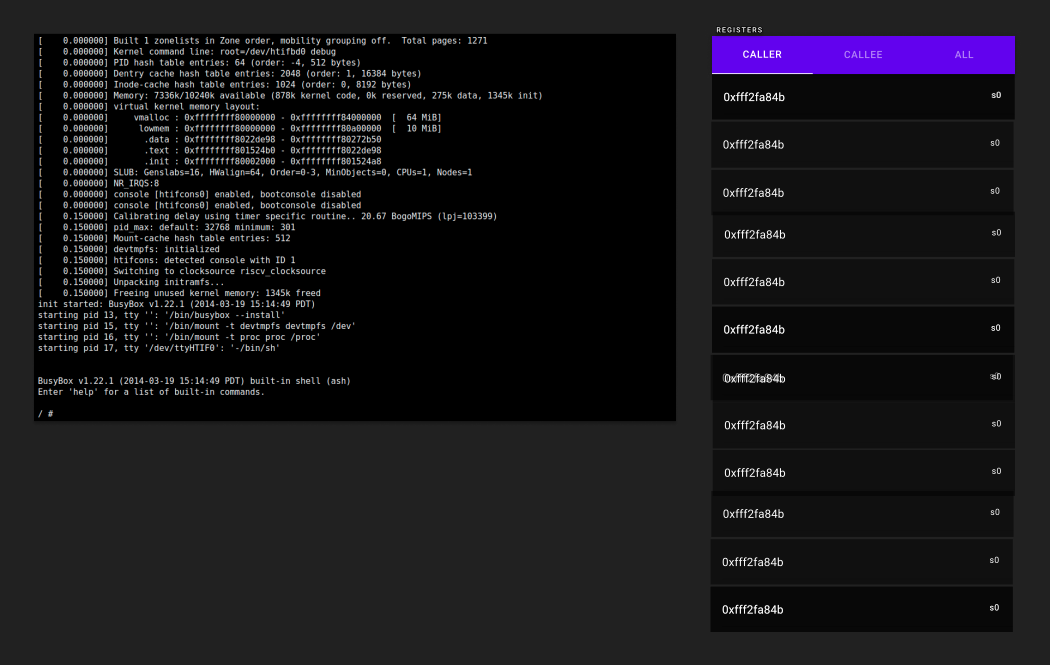
\includegraphics[scale=0.2]{prototype2}
  \caption{Initial prototype using Material Design}
  \label{fig:proto2}
  \centering
\end{figure}

In addition to our team not being expert designers, we are also not experts in CSS, which
is vital to making the application look good. We wanted our application to be as
lightweight as possible, so we wanted to have our own custom CSS, as opposed to using a CSS
framework like Bootstrap. To learn CSS and UI design
patterns further, we read the book \href{https://refactoringui.com/}{Refactoring UI}, which
provided many design tips from a developer's point of view.

We established a design system that is used throughout the app. We defined a system for colors,
fonts, spacing/font size, and more. The system restricts properties of the UI to follow a discrete
set of values. Although at first glance, it may seem that this restriction would limit our ability
to create a design. In fact, the restriction provided by the design system helped to make
the application feel polished and consistent.


%-------------------------------------------------------------------------------
\section{Implementing a Working Prototype}
%-------------------------------------------------------------------------------

\subsection*{A Modular Design}

We describe our app as a modular, dashboard user interface that lets users use a
basic OS and see properties about the OS and CPU in real time.

Our modular design means we have separate components for each visualization in the dashboard.
For example, there is a separate component for the window showing the registers, a separate
component for the view showing the ratio of instructions being executed, and so forth.
We split our app into modular components for several reasons:

\begin{itemize}
  \item easier to maintain and test
  \item allows features to rapidly developed
  \item offers more flexibility in UI structure
\end{itemize}

We will elaborate on each of these points.

First, because our dashboard interface uses modular UI components, whenever we work on a single
component, we can be confident that breaking a single component won't break other parts of the app.

The modular design also allows us to split the work and develop features independently. This is great for
us during these times of quarantine because of COVID-19. So, for example, while one team member is working on some feature
$A$, another team member can be styling feature $B$. And since the components are modular, we can do so without
worrying about conflicting with another person's work.

Finally, having the components act as modular entities allows us to change the layout of the UI very easily should
we choose too. The components are simply independent building blocks that can be moved around as we please. This 
flexibility will become very important when it comes time to finalizing our app.

\subsection*{Finishing our Prorotype}

For our minimum viable product, we have chosen the following features for our dashboard:

\begin{itemize}
  \item show the contents of the 32 user registers
  \item show the ratio of CPU instructions executed
  \item a time series graph showing memory utilization
\end{itemize}

We feel that this offers a useful feature set to get a glance at what is going on under the hood
of an operating system utilizing the RISC-V instruction set.
Figure 2 shows our working prototype which includes these features.

% change this when we have a picture of the prototype
\begin{figure}[H]
  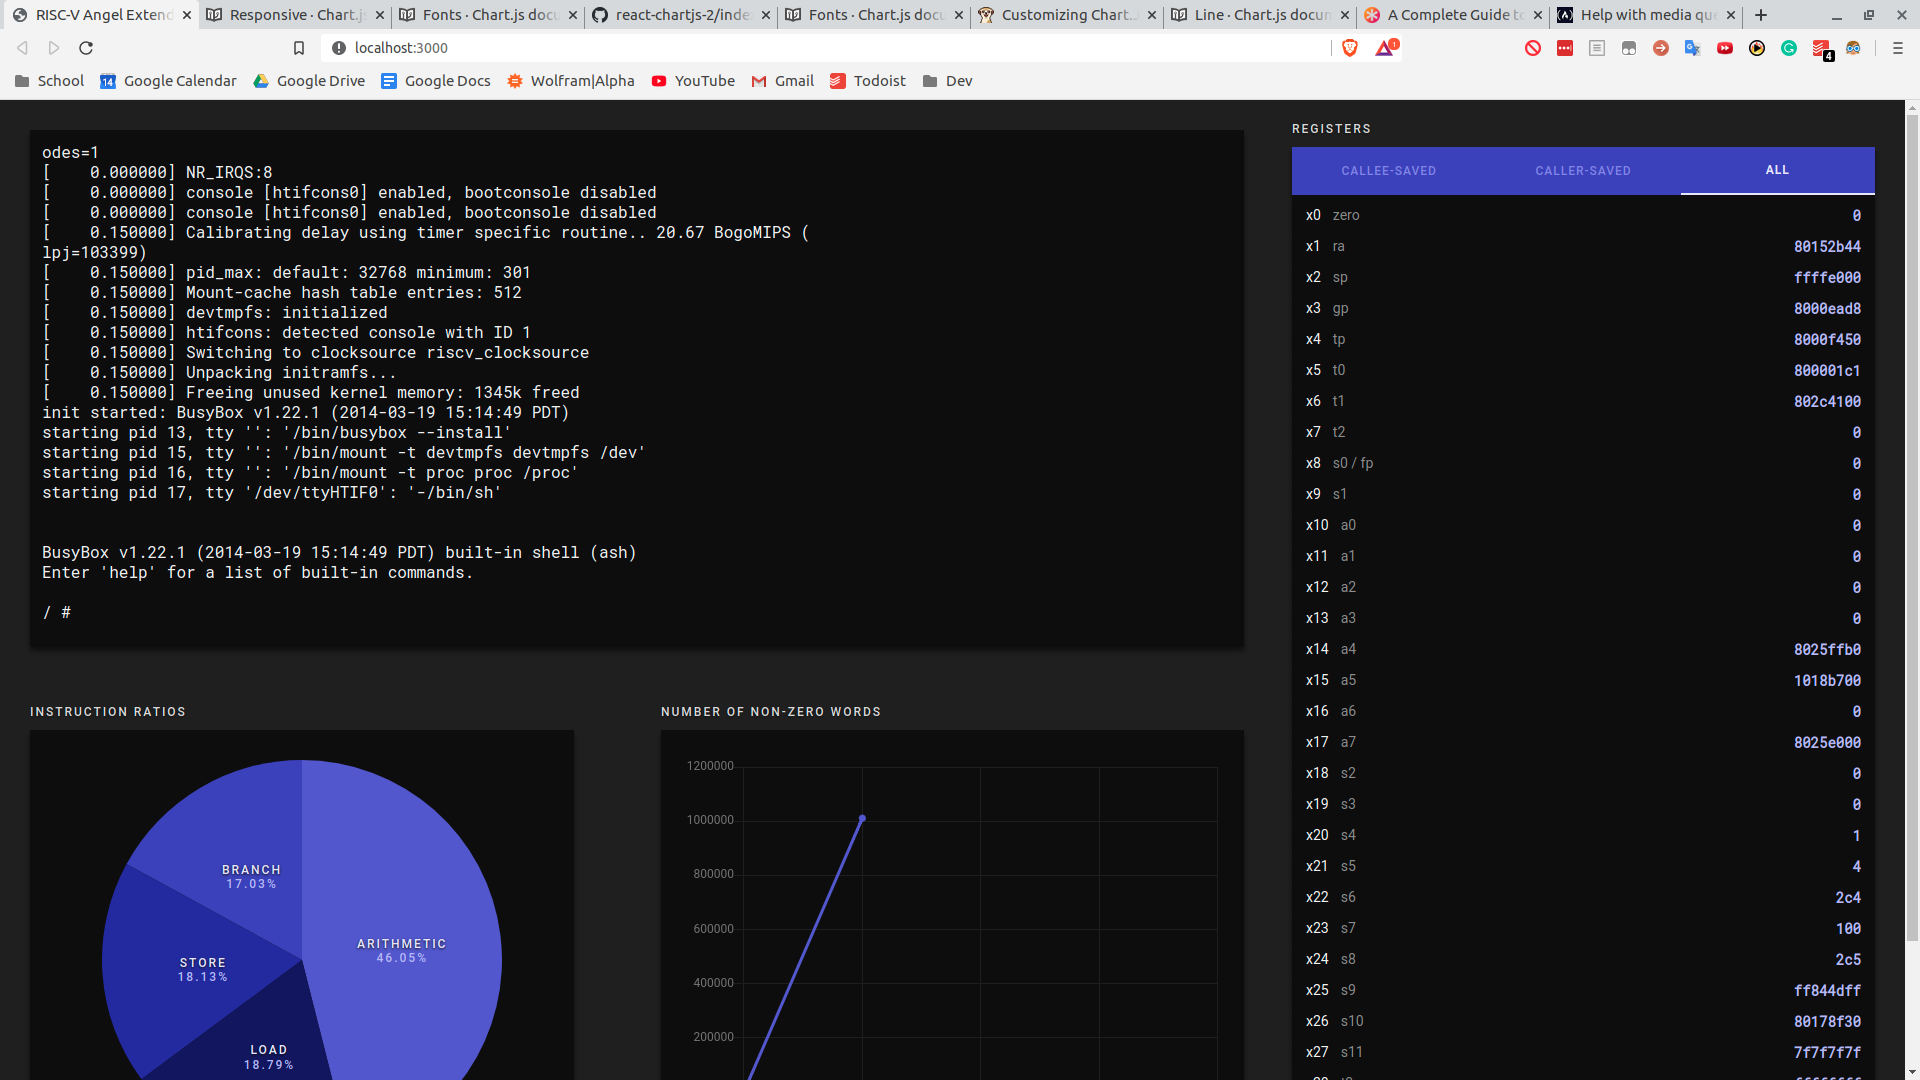
\includegraphics[scale=0.125]{mvp}
  \label{fig:mvp}
  \caption{MVP}
  \centering
\end{figure}

%-------------------------------------------------------------------------------
\section*{Future Plans}
%-------------------------------------------------------------------------------

Before we demo, we plan to

\begin{itemize}
  \item Make our application responsive; right now it only works on desktop screens.
  \item Improve the application performance; try to remove message passing between React code and the VM.
  \item Deploy the application to the web.
\end{itemize}

We have some ideas for potential bells and whistles for our dashboard which include

\begin{itemize}
  \item Allow user to change endianness
  \item Show information about the file system like which files are open
  \item Show information about the processes that running on the OS 

To wrap up the software development lifecycle for this app,
we may open a pull request on the base riscv-angel branch. Hopefully, this
could invoke some inspiration to keep riscv-angel up to date and maintained in the future,
making riscv-angel a tool that can be used by educators and enthusiasts alike to visualize
what goes on under the hood of an operating system.


%-------------------------------------------------------------------------------
\section*{Acknowledgments}
%-------------------------------------------------------------------------------

Thanks to all of the contributors of \href{https://github.com/riscv/riscv-angel}{riscv-angel},
in which this project is based on.

%-------------------------------------------------------------------------------
\section*{Availability}
%-------------------------------------------------------------------------------

This project is open-source and is available at
\href{https://github.com/swkeever/riscv-angel-extended}
{https://github.com/swkeever/riscv-angel-extended}

%-------------------------------------------------------------------------------


%%%%%%%%%%%%%%%%%%%%%%%%%%%%%%%%%%%%%%%%%%%%%%%%%%%%%%%%%%%%%%%%%%%%%%%%%%%%%%%%
\end{document}
%%%%%%%%%%%%%%%%%%%%%%%%%%%%%%%%%%%%%%%%%%%%%%%%%%%%%%%%%%%%%%%%%%%%%%%%%%%%%%%%

%%  LocalWords:  endnotes includegraphics fread ptr nobj noindent
%%  LocalWords:  pdflatex acks
